\chapter{Analise do problema e desenho de uma solução}
\label{chap:analisedoproblema}

\textit{Adicionar texto introdutorio}

\section{O Dominio}

Este projeto tem como objetivo a criação de uma plataforma adaptada à organização e aos seus desafios. Para tal, foi necessário esquematizar a respetiva lógica de negócio.

Após discussões 

\begin{figure}    
    \centering
    %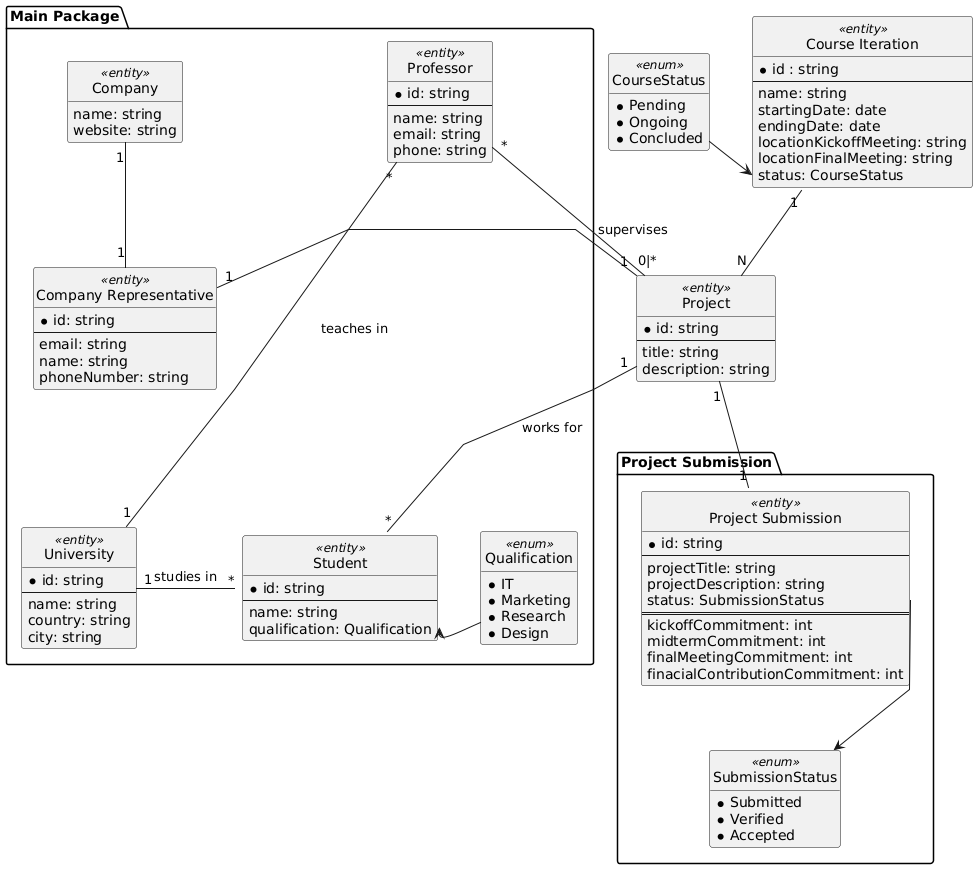
\includegraphics[width=\pagewidth]{capitulos/cap3-analisedoproblema/assets/entity-diagram/cd.png}
    \caption{Diagrama de classes da lógica de negócio do Blended4Future 1}
    \label{fig:cd}
\end{figure}


\section{Engenharia de requisitos}

Durantes os primeiros dois sprints foi estabelecido um \textit{backlog} de \textit{user stories} que refletia as funcionalidades necessárias


\subsection{User Flow Chart}

\subsection{Requisitos funcionais}

\subsubsection{Casos de uso}

\subsection{Requisitos não Funcionais}

incluir tambem a necessidade de CI/CD Pipelines


\section{Arquitetura do sistema}

\subsection{Desenho do sistema}

\subsection{Nivel 1}

\subsection{Nivel 2}

\subsection{Nivel 3}

\subsection{Nivel 4 - Código}

\subsection{Padrões utilizados}
